\section{Methodology}
\label{seq:methodology}
In this thesis we will compare 10 models to each other for 3 different time intervals. The models we choose are diverse in the way they work to make better comparisons.\\

We start with one of the most basic statistical methods there is, the Local Level model described in \ref{subsec:state space}. This model tries to explain the data with a local average. Then we add regressor data to the local level model resulting in the regression model described in \autoref{subsec:state space}. To place this thesis better in the literature we will also make an ARIMA model described in \autoref{subsec:arima} as many research exists comparing models to the ARIMA model. As with the Local Level model, we can expand the ARIMA model with regressor data resulting in the ARIMAX model described in \autoref{subsec:arimax}. The Fused Lasso model introduces some temporal awareness and shrinks regressors that are far away from each other in time which we think would be a valuable addition to the already listed models. The fused lasso is further described in \autoref{subsec:flasso}. The two univariate machine learning models we will use are the Artificial Neural Network and extreme gradient boosting models. The Artificial Neural Network uses a Neural Network to model non-linear relationships described in \autoref{subsec:ann} and the XGBoost model constructs a decision tree to make predictions described in \autoref{subseq:xgb}.\\

There are also two multivariate models that use data which is split by skill which is needed to solve the case. To compare the multivariate models with the univariate models, the predictions for the different case types are added together such that we again get the total number of cases from the multivariate models. The underlying assumption is that the multivariate models can discover more patterns in the data and can possibly perform better than their univariate counterparts. To model this we introduce two more models, the statistical VARIMAX model (further described in \autoref{subsec:varimax}) that is a multivariate version of the ARIMAX model, and a multivariate version of the artificial Neural Network.\\

In the following part of the thesis there are a lot of notations so first here is a list of the notation that is used throughout this section: $T =$ The set of all the time points, $t =$ A Single time point, $n =$ The number of dimensions for regressor data $x_{t, i} =$, A regressor value at time $T$ and value $i$, $y_t =$ The dependent data at point t in time, $Y =$ All the dependent Data, $\beta =$ The real coefficient, $\hat{\beta} =$ An estimated coefficient and $|Z||^2_2 = \sum_{t=1}^Tz_t$ 

\subsection{Local Level and Regression Model}
\label{subsec:state space}
The state space representation introduced by \cite{Kalman1960AProblems} is a model that can be represented using the two equations \eqref{eq:general_state_space} defining two variables. The observation vector $y_t$ and the state vector $\alpha_t$.  $y_t$ and $\alpha_t$ form the main parts of the state space representation. $\alpha_t$ stands for the state of the underlying model and $y_t$ is the actual result.

\begin{equation}
\label{eq:general_state_space}
\begin{aligned}
\alpha_{t+1} &= T_t\alpha_t + R_t\zeta_t \quad &\zeta_t \sim \mathcal{NID}(0, Q_t)\\
    y_t &= Z_t\alpha_t + \epsilon_t \quad &\epsilon_t \sim \mathcal{NID}(0, H_t)
\end{aligned}
\end{equation}

%\subsubsection{Kalman filter}
%\label{subsec:Kalman filter}
with parameters $T_t$, $R_t$, $Q_t$, $Z_t$, $H_t$ and $\alpha_t$ that need to be defined by the model that is represented in State Space. To update the state vector $\alpha_t$ the Kalman filter \citep{Kalman1960AProblems} can be used. The Kalman filter uses a set of equations \eqref{eq:kalman_equations} to update $\alpha_t$.

\begin{equation}
\label{eq:kalman_equations}
\begin{split}
    v_t &= y_t - Z_t a_t\\
    f_t &= Z_t P_t Z_t' + H_t\\
    K_t &= T_t P_t Z_t' F_t^{-1}\\
    a_{t+1} &= T_t a_t + K_t v_t\\
    P_{t+1} &= T_t P_t T_t' + R_t Q_t R_t' - K_t F_t K_t'\\
\end{split}
\end{equation}
With $v_t$ as the prediction error, $f_t$ as the variance of the prediction error and $K_t$ as the Kalman gain. With variance $P$ and state vector $a$ defined as:
\begin{equation*}
\begin{split}    
    a_{t+1} &= \mathbb{E}(\alpha_{t+1}|Y_t)\\
    P_{t+1} &= \mathbb{V}\text{ar}(\alpha_{t+1}|Y_t)
\end{split}
\end{equation*}
To make good estimates for our parameters, the loglikelihood is minimized using the L-BFGS-B method. The parameters which can be minimized can differ depending on the model that is represented in State Space. The loglikelihood equation is described in equation \ref{eq:kalman_loglikeli}
\begin{equation}
    \log \mathcal{L} = -\frac{n}{2} - \frac{1}{2}\sum\limits_{t=1}^n \log|F_t| - \frac{1}{2}\sum\limits_{t=1}^n v_t' F_t^{-1} v_t
\label{eq:kalman_loglikeli}
\end{equation}
Further descriptions and derivations can be found in \cite{Durbin2012TimeModels}\\
%\subsubsection{Kalman Smoother}
%An issue with the Kalman filter is that only the variables until $t$ ($[1:t]$) are taken into account and not the complete state vector $T$. This lead to results with larger differences and forecasts that do not take into account the variables that are being calculated later. The solution to this is the Kalman Smoother which uses a backward recursion on Kalman filter estimates which means that all the values $[1:T]$ are taken into account. The state smoothing algorithm is given by:
%\begin{equation}
%\begin{split}
%    L_t &= T_t - K_tZ_t\\
%    r_{t-1} &= Z_t'v_t + L_t'r_t\\
%    N_{t-1} &= Z_t'F^{-1}Z_t + L_t'N_tL_t\\
%    \alpha_t &= a_t + P_t r_{t-1}\\
%    V_t &= P_t - P_t N_{t-1} P_t\\
%\end{split}
%\end{equation}
%where we then have
%\begin{equation*}
%\begin{split}
%    \alpha_t &= \mathbb{E}(\alpha_t|Y_n)\\
%    V_t &= \mathbb{V}ar(\alpha_t|Y_n)
%\end{split}
%\end{equation*}
%Further descriptions and derivations can be found in \cite{Durbin2012TimeModels}
%}

%\subsection{Local Level Model}
The first model in state space representation that will be used in this thesis is the local level model. The local level model estimates the variance parameters of the state space vector and the state variable. The local level model gives us an idea about where the local average is. This model does not take much input parameters and can give us an idea about how a very simple model would perform in this data set as well as giving us a good starting point to start with our analysis with a model that has not many parameters. The local level model estimates the variance of the error terms as $\sigma_{\epsilon}^2$ and the variance of the state space equation $\sigma_{\eta}$. The local level model is given in state space form as:
\begin{equation}
\begin{split}
    y_t &= \alpha_t + \epsilon_t, \quad \epsilon_t \sim N(0,\sigma_\epsilon^2)\\
    \alpha_{t+1} &= \alpha_t + \eta, \quad \nu_t \sim N(0, \sigma_\eta^2)\\
\end{split}
\end{equation}
The Local level model is estimated using a Kalman Filter on the state space model with Z = 1, T = 1, R = $\sigma_\eta^2_t$, H = $\sigma_\epsilon^2$ \\

%\subsection{Regression model}
A first expansion of the local level model is to incorporate explanatory data in the model. A good explanatory data set helps the model find patters in the data which can help in making a forecast of the dependent variable. This model with explanatory data is the regression model.  The regression model can also be written in state space form. The regression model finds linear relationships between the explanatory data X and the dependent variable Y. The regression model is defined by:$$y_t = X_t\beta + \epsilon_t$$ and can be represented in state space form and estimated with a Kalman Filter as well. The state space representation of the regression model can be seen in equation \ref{eq:regression_state_space}. Where $\alpha^*$ is the new state space vector and $I_d$ is the Identity matrix.\\

\begin{equation}
    a^*_t = \left(\begin{array}{c} \beta \\ a_t \end{array} \right) \quad
    T = I_{d+1} \quad
    R = \left[\begin{array}{c} 0 \\ \sigma_\eta^2\\\end{array}\right] \quad
    Z = \left[\begin{array}{c c c c}
        x_{1,1} & \hdots & x_{1,n} &  1 \\
        \vdots &  \ddots& \vdots & \vdots \\
        x_{t,1} & \hdots & x_{t,n} & 1 \\
    \end{array}\right]
\label{eq:regression_state_space}
\end{equation}

\subsection{The ARIMA family}
Autoregressive models are models that do a 'simple' regression on their own lags. The ARIMA family of models are models based on the ARIMA (AutoRegressive Integrated Moving Average) model. Autoregressive means it regresses on the lags of the dependent variable. Integrated means it can handle integrated data and the moving average means it has a moving average component.

\subsubsection{ARIMA}
\label{subsec:arima}
The first model we want to consider from the ARIMA family is the ARIMA(p,d,q) model. This model is well studied in literature and one of the reasons we want to include this model in this thesis is that there exist many studies comparing other models we use in this thesis to the ARIMA model. To be able to better place the results of this thesis in literature the ARIMA model is included. The ARIMA model is a linear combination with lags and a moving average component. The ARIMA model assumes linear relationships of the dependent variable with its own lags. The model has p lags, is differentiated d times and has q moving average components. The ARIMA(p,d,q) model is defined in \autoref{eq:arima} with $p$ as the number of lags, $d$ as the order of differencing in the ARIMA model, q as the number of moving average components, $\bar{y}$ as the differenced value of $y$ and $\theta_j$ as the j'th moving average component with $j \in \{1, ..., q\}$.
\begin{equation}
\begin{split}
    \tilde{y}_t &= y_t - y_{t-d}\\
    \tilde{y}_t &= \sum\limits_{i=1}^p \beta_i \tilde{y}_{t-i}  + \sum\limits_{j=1}^q \theta_j \epsilon_{t-1}
\label{eq:arima}
\end{split}
\end{equation}
The parameters of the ARIMA model will be estimated using the L-BFGS-B method \citep{L-BFGS-B} to minimize the least squares function of $S_{\text{least Squares}} = \sum^n_{i=1} (Y - \hat{Y})^2$.

\subsubsection{ARIMAX}
\label{subsec:arimax}
The approaches of the ARIMA model and the regression model can be combined to form the ARIMAX model. The ARIMAX model is an extension of the ARIMA model. The full name of the ARIMAX model is the Autoregressive Integrated Moving Average with Explanatory Data. The ARIMAX model incorporates some lags of the dependent data Y and some moving average components as in the ARIMA model. The ARIMAX model differs from the ARIMA model as it incorporates a set of the explanatory data X in the model as some patterns might be explained by this data and not only from the lags. $\gamma$ represents the coefficients corresponding to the explanatory data X.\\

\begin{equation}
\begin{split}
    \tilde{y}_t &= y_t - y_{t-d}\\
    \tilde{y}_t &= \sum\limits_{i=1}^p \beta_i \tilde{y}_{t-i}  + \sum\limits_{j=1}^q \theta_j \epsilon_{t-1} + \Gamma X_t\\
    \Gamma &= \left[\begin{array}{c} \gamma_1 \\ \vdots \\ \gamma_b \end{array}\right] \quad X_t = \left[ \begin{array}{c} x_{1,t}\\ \vdots\\ x_{n,t} \end{array} \right]
\end{split}
\end{equation}
Where $b$ is the dimensionality of the explanatory data X. The ARIMA as well as the ARIMAX models are further described by \cite{Kirchgassner2013IntroductionAnalysis}. The parameters of the ARIMAX model are estimated by the L-BFGS-B method \citep{L-BFGS-B} that minimises the sum of the squared errors of the sample prediction.

\subsubsection{VARIMAX}
\label{subsec:varimax}
Because we are dealing with lags and explanatory data in this model, it might be possible to expose and describe more patterns in the data if we split the data by case skill type as a drop in temperature might have a faster or different effect on senior phone cases than on assortment suggestions. To test if this approach yields better results than directly trying to forecast the total number of cases we introduce the VARIMAX (Vector Autoregressive Integrated Moving Average with Explanatory data) model. The VARIMAX model is an extension of the ARIMA and ARIMAX models that predicts multivariate data. For the purpose of this thesis we will take the sum of the outcomes of the VARIMAX model such that we get the Total Number of Cases. The VARIMAX model is given in \autoref{eq:VARIMAX}. Because of the large number of parameters $\theta$, $\beta$ \& $\gamma$, the least squares cannot be optimized using the L-BFGS-B method, but it will be minimized instead using the SLSQP method \citep{SLSQP}.
\begin{equation}
\begin{split}
    \tilde{Y}_t &= Y_t - Y_{t-d}\\
    \tilde{Y}_t &= \sum\limits_{i=1}^p B_i \tilde{Y}_{t-i}  + \sum\limits_{j=1}^q \theta_j \epsilon_t +  \Gamma X_t\\
    Y_t &= \left[\begin{array}{c} y_{1,t}\\ \vdots \\ y_{l, t}\end{array}\right] \quad B_i = \left[\begin{array}{c} \beta_{1, i} \\ \vdots \\ \beta_{l,i} \end{array}\right] \quad \Gamma_k = \left[\begin{array}{c c c}
        \gamma_{1, 1} & \hdots & \gamma_{1, b}\\
        \vdots & \ddots & \vdots\\
        \gamma_{l, 1} & \hdots & \gamma_{l, b}\\
    \end{array}\right]\\
    X_t &= \left[\begin{array}{c c c}
        x_{1, 1, t} & \hdots & x_{1, b, t}\\
        \vdots & \ddots & \vdots\\
        x_{l, 1, t} & \hdots & x_{l, b, t}\\
    \end{array}\right]
\end{split}
\label{eq:VARIMAX}
\end{equation}
\subsection{Fused Lasso}
\label{subsec:flasso}
The fused LASSO \citep{Tibshirani2005SparsityLasso} is based on the lasso \citep{Tibshirani1996RegressionLasso}. The Fused LASSO penalises coefficients that have a large euclidean distance between each other. This might be beneficiary for a forecast as it prevents outliers and penalises large differences in the coefficients. Both the fused lasso and the lasso try to predict a linear model. The LASSO finds the coefficients with the least squared estimation: $$\hat{\beta}_{LASSO} = \min \left\{\frac{1}{T}||Y - X\beta||_2^2\right\}\quad \text{subject to} \quad \sum_j|\beta_j| \leq s_1$$
A problem with this approach is that it does not take into account temporal data. This is important as the data points close to the variables we want to predict might hold much more value than other data points. The fused lasso aims to fix this problem by introducing a new constraint to the minimisation problem which transforms the estimation to: 
\begin{equation}
\label{eq:fusedlasso}
  \begin{gathered}
    \hat{\beta}_{LASSO} = \min\limits_{\beta} \left\{\frac{1}{T}||Y - X\beta||_2^2\right\}\\
    \text{subject to} \\
    \sum_j|\beta_j| \leq s_1 \text{and} \sum^n_{j=2}|\beta_j-\beta_{j-1}|\leq s_2
\end{gathered}
\end{equation}
where $s$ is the sparsity parameter. $s_1$ penalises the regressors if they have a large value of $\beta$ which makes sure variables which contribute little to the models will receive a small value of $\beta$. $s_2$ encourages values of $\beta$ to be close to each other and penalise $\beta$'s that are far apart. The minimization problem that comes from \eqref{eq:fusedlasso} can be solved by the penalised least squared criterion. \cite{Knight2000AsymptoticsEstimators} describe the asymptotic properties for the lasso which are similar for the fused lasso. The penalised least squared criterion for the fused lasso is given in equation \eqref{eq:lassominimised} which can be minimized.
\begin{equation}
    \label{eq:lassominimised}
    \sum\limits_{i=1}^T (y_t - x_t^T\beta)^2 + \lambda^{(1)} \sum\limits^n_{j=1} |\beta_j| + \lambda^{(2)}\sum\limits^n_{j=2} |\beta_j - \beta_{j-1}|
\end{equation}
The selection of $\lambda^{(1)}$ and $\lambda^{(2)}$ is done using the leave-one-out cross-validation described in \cite{Hwang2016CrossAcceleration, Cawley2003EEcientClassifiers}

\subsection{Extreme Gradient Boosting (XGBoost)}
\label{subseq:xgb}
The first machine learning model that is included in this thesis is the XGBoost model. XGBoost is a gradient boosted tree method introduced by \cite{Chen2016XGBoost:System}. A tree method is a model that makes use of decision trees to come to a prediction. A graphical representation of a decision tree can be found in figure \ref{fig:decission_graphic} where the simple idea for a regression tree is represented with leaves and decision nodes. The XGBoost builds multiple decision trees and takes the average of these trees as the final outcome. The XGBoost has the objective to predict the outcome of
\begin{equation}
\label{eq:xgbpredictionfunc}
    \hat{y}_y = \phi(x_i) = \sum\limits_{k=1}^K f_k(x_i), \quad f_k \in \mathcal{F}
\end{equation}
where $\mathcal{F} = \{f(x)=w_{q(x)}(q:\mathbb{R}^m \to T, w \in \mathbb{R}^T)$, q maps the value to the corresponding leaf index, K is the number of additive function in the model, L is the number of leaves in the tree and $f_k$ corresponds to a leaf tree structure with leaf weights $w$. The function has no mathematical solution. Therefore the model is trained using the additive method in \eqref{eq:ministatxgboost} which penalises the outcome depending on the distance between real values and the estimated value and a regularisation term defined in \ref{eq:xgbpenalization}.
\begin{equation}
\label{eq:ministatxgboost}
\begin{gathered}
    \mathcal{L}^{(t)} = \sum\limits_{i=1}^T l(y_t, \hat{y}_t^{(t-1)} + f_t(x_t)) + \Omega(f_t)
\end{gathered}
\end{equation}
Here $l$ is a differentiable convex loss function which measures the distance between $\hat{y}_i$ and $y_i$. The $\Omega$ function penalises the model complexity and is defined in \eqref{eq:xgbpenalization}. This regularization term helps preventing overfitting and makes gives larger weights to models with a less deep tree.
\begin{equation}
\label{eq:xgbpenalization}
    \Omega(f) = \gamma L + \frac{1}{2} \lambda ||w||^2
\end{equation}
where $\lambda$ is a regularization term to avoid overfitting and $\gamma$ is the threshold parameter for adding notes such that nodes are only added to the tree if the gain is larger than $\gamma$. To be able to quickly optimize this function, the second order tailor approximation is used. The constant is removed such that the objective is simplified.
\begin{equation}
\label{eq:xgbminitailor}
    \mathcal{L}^{(t)} \approx \sum\limits_{i=1}^n[g_if_t(x_i) + \frac{1}{2}h_if_i^2(x_i)] + \Omega(f_t)
\end{equation}
with $g_i = \partial_{\hat{y}(t-1)}l(y_i,\hat{y}^{(t-1)})$ and $h_i = \partial^2_{\hat{y}(t-1)}l(y_i, \hat{y}^{(t-1)})$. Then if the structure of the tree is fixed, an optimal weight $w_j^*$ can be calculated for the leaf $j$ with
$$w_j^* = - \frac{\sum_{i\in I_j}g_i}{\sum_{i \in I_j} h_i + \lambda}$$
which has the corresponding value of 
\begin{equation}
\label{eq:xgbscorefunc}
    \tilde{\mathcal{L}}^{(t)}(q) = - \frac{1}{2} \frac{\left(\sum_{i \in I_j} g_i \right)^2}{\sum_{i \in I_j} h_i + \lambda}
\end{equation}
the value of the optimum weights for a tree in \eqref{eq:xgbscorefunc} can be used as a score function for tree $q$. However, because of computational constraints it is usually infeasible to evaluate \eqref{eq:xgbscorefunc} for all possible trees $q$. To avoid this problem, an algorithm that starts from a leaf and then adds branches is used. This algorithm then needs a split function that evaluates the split such that the algorithm can compare the splits and choose the best split. The split function used with $I = I_L \cup I_R$ is defined in \ref{eq:xgbsplitfunc}. 
\begin{equation}
\label{eq:xgbsplitfunc}
    \mathcal{L}_{split} = \frac{1}{2}\left[ \frac{\left(\sum_{i\in I_L} g_i\right)^2}{\sum_{i\in I_L}h_i + \lambda} + \frac{\left(\sum_{i\in I_R} g_i \right)^2}{\sum_{i\in I_R}h_i + \lambda} - \frac{\left(\sum_{i\in I}g_i\right)^2}{\sum_{i\in I}h_i + \lambda}\right] - \gamma
\end{equation}
The equation \eqref{eq:xgbsplitfunc} is also known as the gain function. To find the split it is not computationally feasible to use a greedy algorithm that tries every different solution. Therefore this algorithm will use the Sparsity-aware Split Finding algorithm \citep{Chen2016XGBoost:System} to build the tree.
\subsection{Artificial Neural Network}
\label{subsec:ann}

\begin{figure}
    \begin{subfigure}{.5\textwidth}
        \centering
        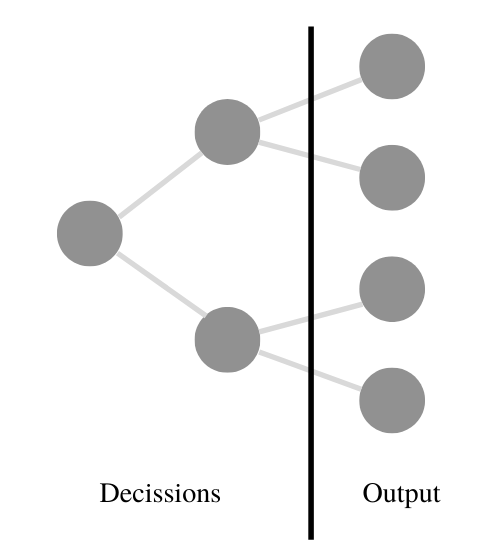
\includegraphics[width=.7\linewidth]{pics/Decission Tree.png}
        \caption{Decision tree}
        \label{fig:decission_graphic}
    \end{subfigure}%
    \begin{subfigure}{.5\textwidth}
        \centering
        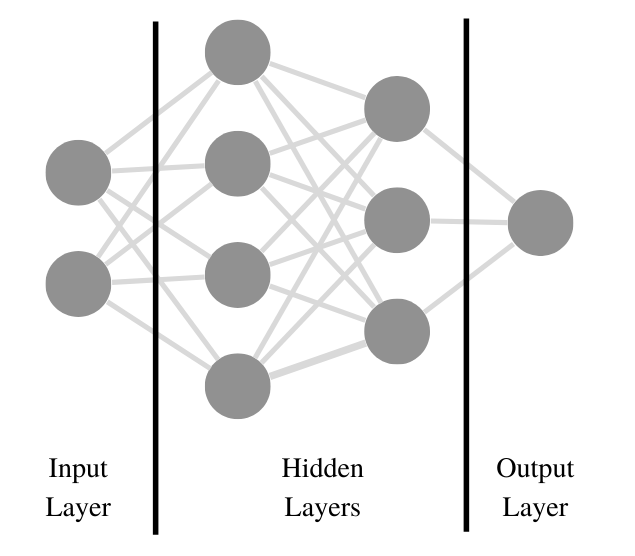
\includegraphics[width=.9\linewidth]{pics/Neural Network.png}
        \caption{Neural network}
        \label{fig:nn_graphic_representation}
    \end{subfigure}
    \centering
    \caption{A graphical representation of the models}
    \label{fig:graphical_representation}
\end{figure}

The second machine learning method we will use in this thesis is an artificial neural network. Because the neural network works in a very different way than the XGBoost model, it would diversify the selection of models in this thesis. The neural network for regression purposes was proposed by \cite{Specht1991ANetwork}. A neural network is a structure that uses one or multiple hidden layers to make a non-linear transformation which is loosely based on biological neural systems. The network consists of multiple layers performing operations and together they form the network. The three different types of layers in a neural network are the input layer, the hidden layers and the output layer. The input layer consists of the inputs $X = \{x_1, x_2, ..., x_d\}$ which are the regressors. There can only be one input layer. The hidden layers form linear combinations between the input layer, other hidden layers and the output layer. These linear combinations together will make a non-linear function. There can be multiple hidden layers. The output layer is the final layer where the dependent variables $Y = \{y_1, ..., y_d\}$ are formed. There can only be one output layer.\\

A graphical representation of these layers in a simplified form can be found in figure \eqref{fig:nn_graphic_representatio}. In this figure, one can clearly see the difference with the tree structure in \eqref{fig:graphical_representation} as there the neural network consists of multiple linear combinations combining to the answer in the end while the tree structure has multiple possible but fixed end answers. Between the layers, the function $f(x) = w_2 g(w_1^T x + b_1) + b_2$ is used. Where $\{w_1, w_2, b_1, b_2\} = \theta, w_1 \in \mathbb{R}^n \text{ and } w_2, b_1, b_2 \in \mathbb{R}$ are the function parameters. The function $g(\cdot): \mathbb{R} \to \mathbb{R}$ is the activation function defined in \eqref{eq:nn_activationfunction}
\begin{equation}
\label{eq:nn_activationfunction}
    g(z) = \frac{e^z - e^{-z}}{e^z + e^{-z}}
\end{equation}
To be able to estimate the network, backpropagation is used which tries to decrease the loss function. In every iteration, after the Loss function of the output layer is calculated, the backpropogation makes backward passes which updates the previous layers with new weights to decrease the loss function. To calculate the updated weights the L-BFGS function is used \citep{Liu1989OnOptimalization}.
\begin{equation}
    Loss(\hat{y}, y, W) = \frac{1}{2n} \sum\limits_{i=0}^n ||\hat{y}_i - y_i||^2_2 + \frac{\alpha}{2n} ||W||^2_2
\end{equation}
This thesis will use the Scikit-learn implementation of the neural model described by \cite{Pedregosa2011Scikit-learn:Python}.\\

There will also be a multivariate implementation of the neural network where the data is broken down by skill level as is also done with the VARIMAX model. The main difference of the multivariate neural network with the univariate version is that the multivariate model has multiple nodes at the output layer, resulting in a multivariate output.

\subsection{Mixed modeled Forecast}
\label{subseq:mixed model}
If we have a model $S$ which produces an output $X_s$, the output of different models $\{S_1, ..., S_n\}$ might be combined into a mixed model that outperforms all the individual models in S. In this case the mixed model $S_{\text{Mixed}}$ would look like:
\begin{equation}
    S_{\text{Mixed}}: Y_{\text{Mixed}} | X = \sum\limits_{i=1}^n \beta S_i(X)
\end{equation}
Where S is a model that produces a output Y for given data X. $\beta$ is estimated via the least squares method with X as the h ahead forecast from the selected models and Y as the true dependent. This method is shown to improve the individual forecasts that are taken into account and works better when the forecasts in $S_n$ are diverse \citep{Yang2004CombiningResults}. Because we have a lot of forecasts that are generalisations of other models, the models that will be used for this ensemble model are the Fused Lasso model, the XGBoost model, the Artificial Neural Network and the ARIMAX Model.
 
\subsection{Comparing Forecasts}
To know what forecast is the best one, we need to be able to compare them to each other. There are of course the normal measures of quality like MAE (Mean Absolute Error), MSE (Mean Squared Error), MAPE (Mean Absolute Percentage Error) and RMSE (Rooted Mean Squared Error) which will be computed for all the methods that are tested. The mathematical definitions of these measures of quality are described in \autoref{app:measures_of_quality}. To draw statistical significant conclusions we use the Diebold-Mariano test \citep{Diebold1995ComparingAccuracy} in combination with these benchmarks. The Diebold-Mariano test looks to evaluate the accuracy of two forecasts. Define the loss differential as: 
\begin{equation}
    d_t = g(e_{1t}) - g(e_{2_t})
    \label{eq:defferenctial_loss}
\end{equation}
Where $g(\cdot)$ is a loss function for these forecast errors which can be the MSE, MAE, MAPE, RMSE or any other information criterion. The test then seeks to verify the hypothesis defined by:
\begin{equation*}
\begin{split}
    \text{H}_0 : \mathbb{E}(d_t) &= 0 \quad \forall t\\
    \text{H}_1 : \mathbb{E}(d_t) &\neq 0 \quad \forall t\\
\end{split}
\end{equation*}
Where the null hypothesis means that the forecasts have the same accuracy while the alternative hypothesis states that the forecasts have different levels of accuracy. To construct the test statistic we need the population mean of the loss differential or:
\begin{equation*}
    f_d(0) = \frac{1}{2\pi} \left(\sum\limits_{k=-\infty}^\infty \gamma_d(k)\right)
\end{equation*}
Where $\gamma(k)$ is the autocovariance of the loss differential at lag $k$. This can be estimated with:
\begin{equation}
    \hat{f}_d(d) = \frac{1}{2\pi} \left(\hat{\gamma}_d(0) + 2 \sum\limits_{k=1}^{h-1} \hat{\gamma}_d(k)\right), \quad h > 1
\label{eq:loss_diff_hat}
\end{equation}
Where $h$ is the number of steps forecasts. By combining equations \ref{eq:defferenctial_loss} and \ref{eq:loss_diff_hat} we get the test statistic in equation \ref{eq:driebold_mariano_test_statistic} which is asymptotically N(0,1) distributed.
\begin{equation}
    DM = \frac{\bar{d}}{\sqrt{\frac{2\pi\hat{f}_d(0)}{T}}}
    \label{eq:driebold_mariano_test_statistic}
\end{equation}